
\chapter{Marco teórico} % con la palabra capitulo
\graphicspath{{./../imagenes/}}
\linespread{1.3}
\hypertarget{recursos-sumo}{%
\section{Recursos: SUMO}\label{recursos-sumo}}

Para probar y desarrollar a detalle la arquitectura, es necesario contar
con un entorno de simulación versátil y altamente configurable donde
probar los algoritmos creados en base a nuestras hipótesis. El primer
acercamiento para resolver reste problema fue desarrollar desde cero un
simulador de tráfico, pero ya que esto tiene su propia complejidad y no
el objetivo final al que pretendemos llegar, buscamos otras
alternativas. De entre todas, la que parece ser la solución definitiva
es el simulador de tráfico urbano SUMO. ``\textbf{S}imulation of
\textbf{U}rban \textbf{MO}bility'' (Eclipse SUMO) es un paquete de
simulación de tráfico vial de código abierto, altamente portátil,
microscópico y continúo diseñado para manejar grandes redes viales
\textcite{SUMO2018}. Permite simular cómo una determinada demanda de
tráfico que consiste en vehículos individuales se mueve a través de una
red de carreteras determinada. La simulación permite abordar un amplio
conjunto de temas de gestión del tráfico. Es puramente microscópico:
cada vehículo está modelado explícitamente, tiene una ruta propia y se
mueve individualmente a través de la red. Las simulaciones son
deterministas por defecto, pero hay varias opciones para introducir la
aleatoriedad.

Al tratarse de un paquete, la instalación por defecto incluye varias
aplicaciones, scripts e interfaces aparte de SUMO. Estas aplicaciones se
utilizan para importar y preparar redes de carreteras, así como para
procesar datos para su uso en SUMO.

\hypertarget{caracteruxedsticas-relevantes-de-sumo-para-la-investigaciuxf3n-de-tuxe9cnicas-de-control-de-semuxe1foros.}{%
\subsection{Características relevantes de SUMO para la investigación de
técnicas de control de
semáforos.}\label{caracteruxedsticas-relevantes-de-sumo-para-la-investigaciuxf3n-de-tuxe9cnicas-de-control-de-semuxe1foros.}}

\begin{itemize}
\tightlist
\item
  Incluye todas las aplicaciones necesarias para preparar y realizar una
  simulación de tráfico
\item
  Permite simular desde una solo intersección hasta ciudades enteras
\item
  Altamente configurable a través de archivos XML
\item
  Documentación completa y actualizada de todas las características,
  interfaces y librerías que incluye, así como guías, tutoriales y
  ejemplos de configuración de gran cantidad tópicos.
\item
  Gran cantidad de tipos de vehículos disponibles, entre ellos de
  emergencia (ambulancias) y de autoridad (patrullas).
\item
  Calles de varios carriles con cambio de carril, carriles configurables
  para permitir solo el tipo de tráfico especificado.
\item
  Diferentes reglas de derecho de paso, semáforos
\item
  Incluye interfaces en Python para obtener datos de la simulación en
  tiempo real, así como para controlar aspectos de esta, como los
  semáforos.
\item
  Incluye editor gráfico de rutas y GUI para el simulador.
\item
  Velocidad de ejecución rápida (hasta 100.000 actualizaciones de
  vehículo por segundo en una máquina de 1 GHz)
\item
  Código abierto (EPL)
\end{itemize}

\hypertarget{vista-general}{%
\subsection{Vista general}\label{vista-general}}

\begin{figure}[H]
    \centering
    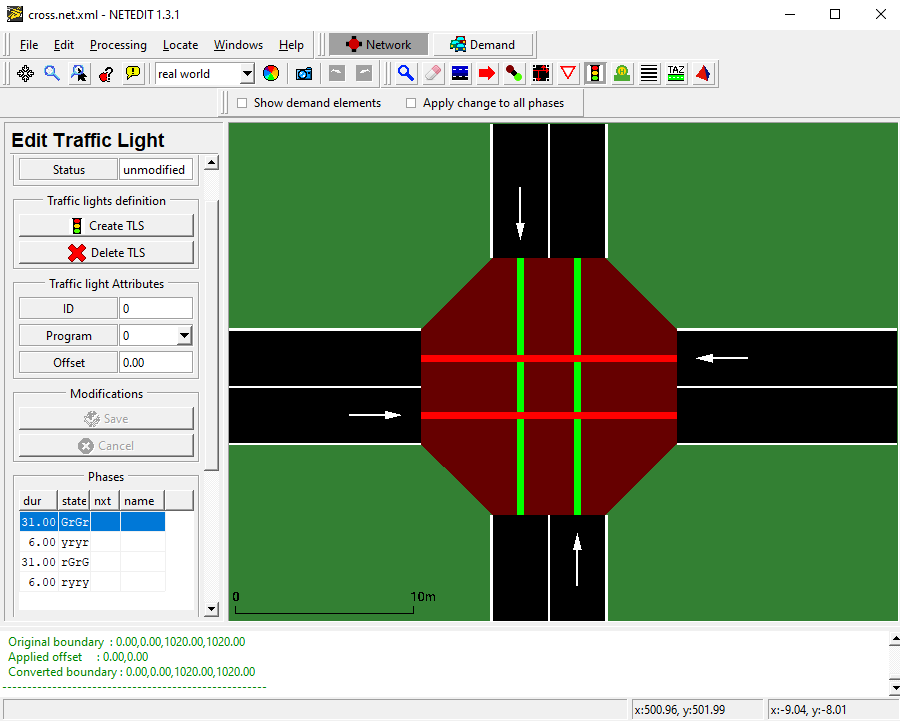
\includegraphics[width=\textwidth]{sumo/1cb8aa292f0be15b402ccd4f098f53e0.png}
    \caption{Editor gráfico NETEDIT mostrando una intersección y el menú de edición de semáforos.}
    \label{fig:netedit1}
\end{figure}

\begin{figure}[H]
    \centering
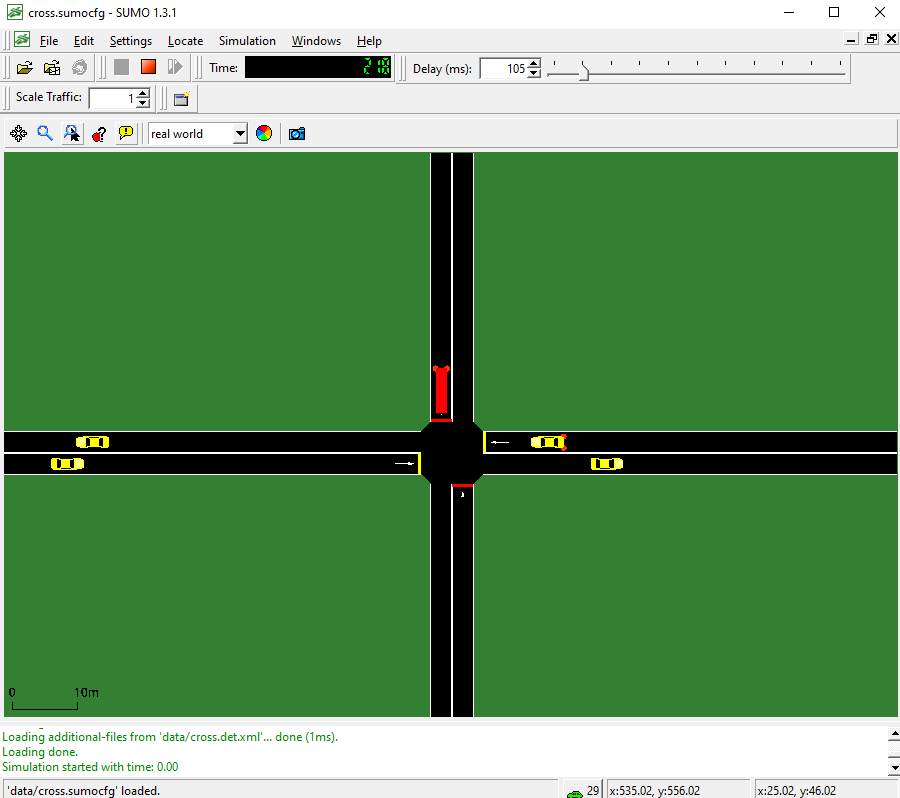
\includegraphics[width=\textwidth]{sumo/f06ad63e2235a639007f9748f2326f91.png}
    \caption{Simulando la intersección anterior de manera gráfica en SumoGui.}
    \label{fig:sumogui1}
\end{figure}

\begin{figure}[H]
    \centering
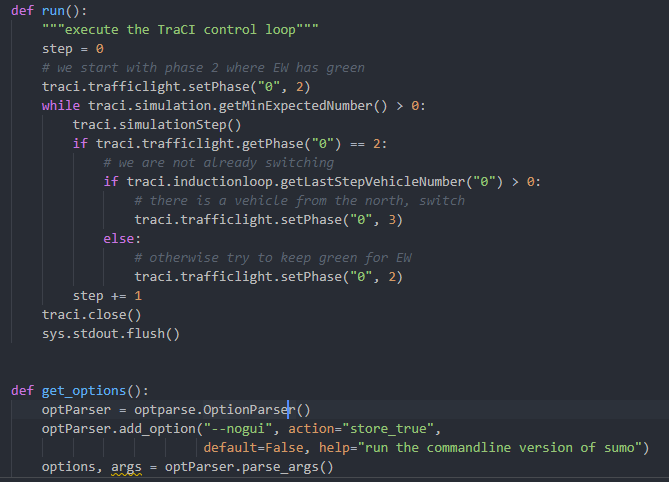
\includegraphics[width=\textwidth]{sumo/8a185a540ef5e98b250d7c70216cddfc.png}
    \caption{Controlando los semáforos desde Python con TraCI (Traffic Control Interface).}
    \label{fig:traci1}
\end{figure}

\begin{figure}[H]
    \centering
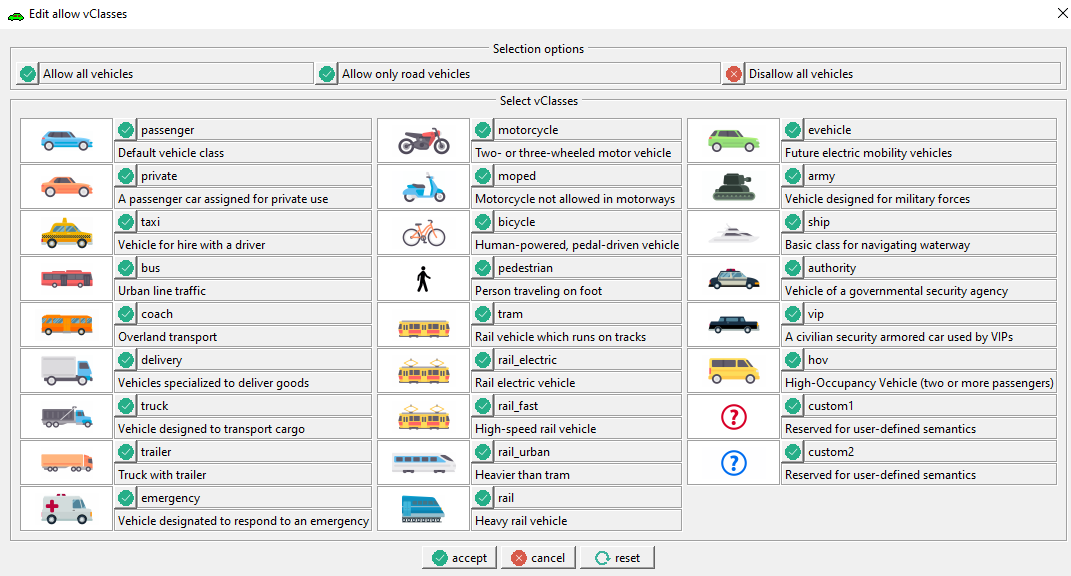
\includegraphics[width=\textwidth]{sumo/d600ef6ce1de01e90d10a436d7b6bb75.png}
    \caption{Los diversos tipos de vehículos disponibles.}
    \label{fig:sumogui2}
\end{figure}

\hypertarget{simulaciuxf3n-de-semuxe1foros}{%
\subsection{Simulación de
semáforos}\label{simulaciuxf3n-de-semuxe1foros}}

Los semáforos (llamados en el simulador TLS - \emph{Traffic Light
System}) se pueden crear de manera gráfica en NETDIT y automáticamente
generan un programa de control.

\begin{figure}[H]
    \centering
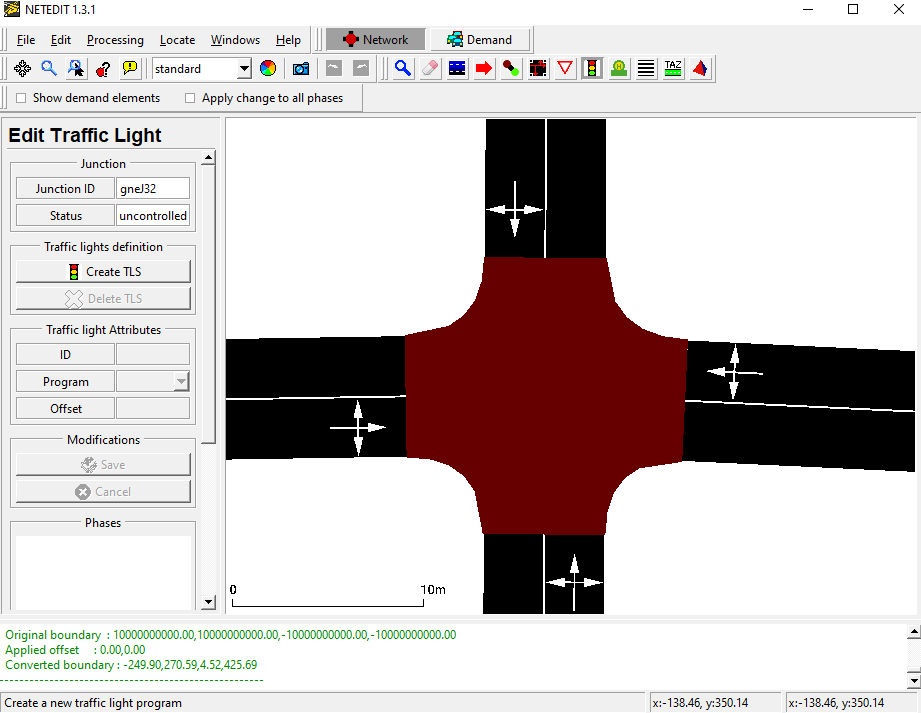
\includegraphics[width=\textwidth]{sumo/d53e12f08f94d08fd7e31f214786b43e.png}
    \caption{Creando gráficamente un programa de control de semáforo en NETDIT.}
    \label{fig:netedit2}
\end{figure}

\begin{figure}[H]
    \centering
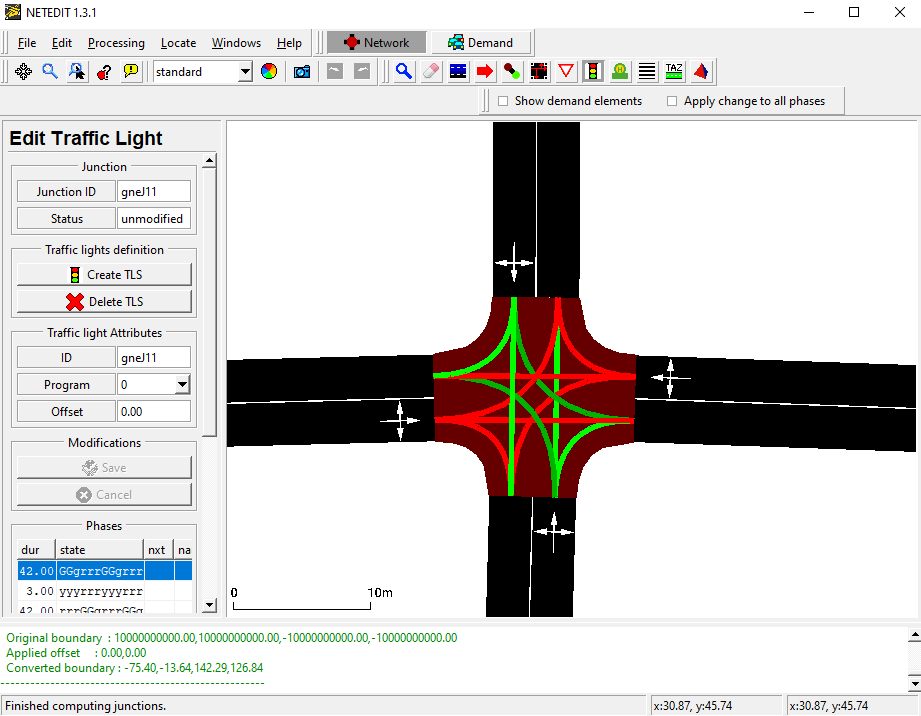
\includegraphics[width=\textwidth]{sumo/e760085ba60c72e71c15ed1d0d5ab9aa.png}
    \caption{Vista gráfica de reglas de paso de un programa de control de
    tráfico en NETEDIT.}
    \label{fig:netedit3}
\end{figure}

\hypertarget{definiciuxf3n-de-nuevos-programas-tls}{%
\subsection{Definición de nuevos programas
TLS}\label{definiciuxf3n-de-nuevos-programas-tls}}

Se puede cargar nuevas definiciones para semáforos como parte de un
archivo adicional. La definición de un programa de semáforo dentro de un
archivo adicional se ve así:

\begin{lstlisting}[language=XML]
<additional>
    <tlLogic id="semaforo_principal" type="static" programID="principal" offset="0">
        <phase duration="40" state="GrGr"/>
        <phase duration="6" state="yryr"/>
        <phase duration="40" state="rGrG"/>
        <phase duration="6" state="ryry"/>
    </tlLogic>
</additional>
\end{lstlisting}

Cada programa está compuesto de varias fases de cierta duración. En cada
una, el atributo \emph{state} define con una cadena de códigos que se
corresponden con los colores de todos los semáforos en esa fase. El
significado de los códigos principales se puede ver en la siguiente
tabla:

\begin{table}[h!]
\centering
\begin{tabular}[t]{c l m{11cm}}
    \toprule
    Código  & Color        & Descripción                                                                                         \\
    \midrule
    r       & rojo         & Luz roja: los vehículos deben detenerse.                                                            \\ 
    y       & amarillo     & Luz amarilla:los vehículos desacelerarán si están lejos de la insersección, de lo contrario pasarán.\\
    G       & verde        & Luz verde de prioridad: los vehículos pasarán.                                                      \\
    \bottomrule
\end{tabular}
\caption{}
\label{table:tab1}
\end{table}

La posiciónde cada caracter en la cadena se corresponde con las
conexiones de la insercción controlada empezando desde arriba en el
orden de las manecillas del reloj. Por ejemplo, la siguiente imagen se
corresponde con la cadena \texttt{state\ =\ "GrGr"}.

\begin{figure}[H]
    \centering
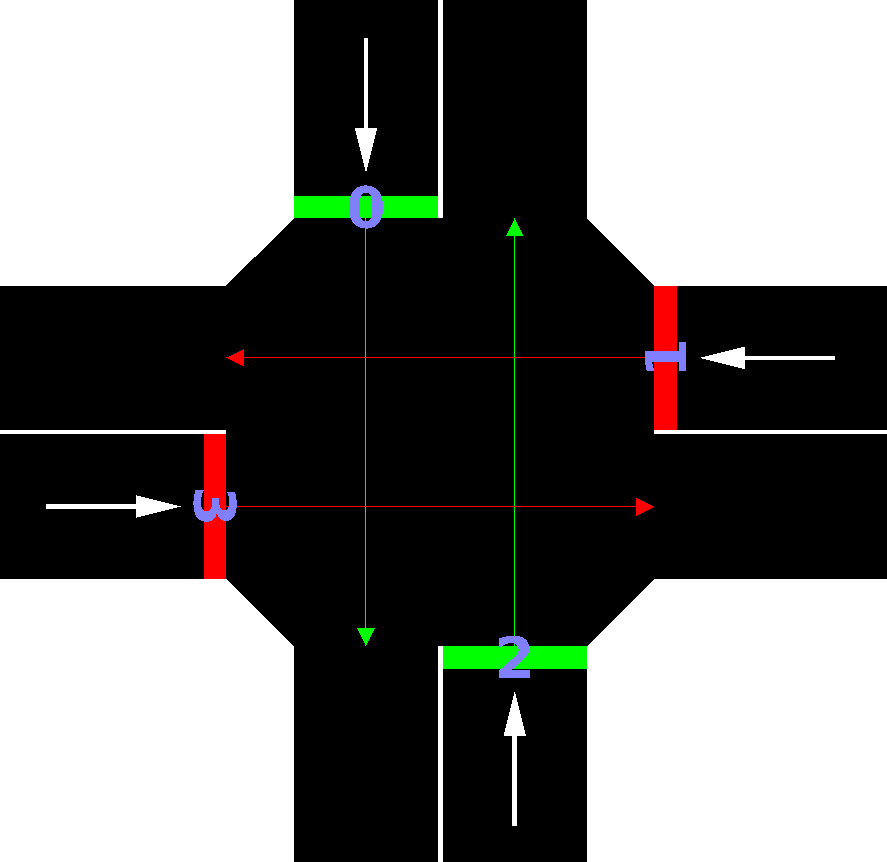
\includegraphics[width=\textwidth]{sumo/tls_light_order.png}
    \caption{Correspondencia de cadenas de códigos a colores de semáforo.}
    \label{fig:netedit4}
\end{figure}

\hypertarget{control-de-los-semuxe1foros-con-python}{%
\subsection{Control de los semáforos con
Python}\label{control-de-los-semuxe1foros-con-python}}

Más importante aún, también es posible controlar los estados de los
semáforos programáticamente a través de una interfaz incluida en el
paquete de instalación llamada TraCI.

TraCI es la abreviatura de
``~\textbf{Tra}fic~\textbf{C}ontrol~\textbf{I}nterface''.~Al dar acceso
a una simulación de tráfico en ejecución, permite recuperar valores de
objetos simulados y manipular su comportamiento ``en línea''.

TraCI utiliza una arquitectura cliente / servidor basada en TCP para
proporcionar acceso a SUMO. De este modo, SUMO actúa como servidor y el
código Python con TraCI como cliente.

A continuación, se muestra el código de ejemplo que controla la lógica
del semáforo para que se controle de la siguiente manera:

\begin{figure}[H]
    \centering
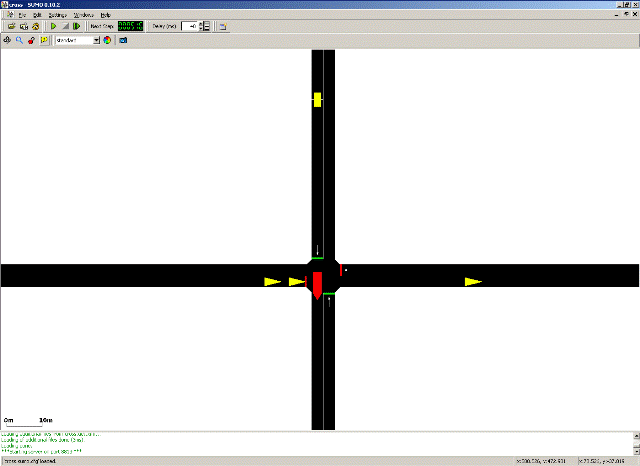
\includegraphics[width=\textwidth]{sumo/3a9d001be95c93c93c1c13ed9aeb7b26.png}
    \caption{Ejemplo de intersección de cuatro vías.}
    \label{fig:sumogui3}
\end{figure}

El ejemplo muestra una simple intersección de cuatro vías. Hay tráfico
normal en el eje horizontal y vehículos importantes (ambulancias,
patrullas, camiones de bomberos, etc.) en el eje vertical de norte a
sur. En la vía que viene desde el norte hay un detector para reconocer a
los vehículos que van entrando. Mientras que ningún vehículo ingresa
desde el norte, siempre damos color verde en el eje horizontal, pero
cuando un vehículo ingresa al circuito del detector, cambiamos la señal
de inmediato para que el vehículo pueda cruzar la intersección sin
detenerse.

\begin{lstlisting}[language=Python]
step = 0
traci.trafficlight.setPhase("0", 2)
while traci.simulation.getMinExpectedNumber() > 0:
    traci.simulationStep()
    if traci.trafficlight.getPhase("0") == 2:
        if traci.inductionloop.getLastStepVehicleNumber("0") > 0:
            traci.trafficlight.setPhase("0", 3)
        else:
            traci.trafficlight.setPhase("0", 2)
    step += 1
traci.close()
\end{lstlisting}

\hypertarget{creaciuxf3n-de-simulaciuxf3n}{%
\section{Creación de simulación}\label{creaciuxf3n-de-simulaciuxf3n}}

Para probar y desarrollar a detalle la arquitectura se usará el
simulador de tráfico urbano SUMO, que incluye prácticamente todas las
herramientas necesarias.

\hypertarget{red-de-carreteras}{%
\subsection{Red de carreteras}\label{red-de-carreteras}}

El primer paso para crear una simulación en SUMO consiste en crear una
red de carreteras. Dichas redes deben estar definidas en un archivo con
extensión .net.xml que puede ser creado de múltiples maneras. Una de
ellas es utilizando la aplicación netconvert (incluida en la instalación
base), que se encarga de importar redes de carreteras de diferentes
fuentes que pueden ser usadas por otras herramientas del paquete
incluído en SUMO. También es posible utilizar la aplicación gráfica
netedit para editar una red previamente creada con netconvert o incluso
crear una desde cero con la misma aplicación.

El método usado para crear la red de carreteras que utilizará la
sumulación es una combinación de los dos anteriores. Se creó la red de
tráfico usando un script llamado
\href{https://sumo.dlr.de/docs/Tutorials/OSMWebWizard.html}{osmWebWizard},
que permite seleccionar un área geográfica real desde OpenStreetMaps y
convertirla en el red con extensión .net.xml que utiliza SUMO.

Para motivos de prueba, se usó una intersección de Mérida conocida, para
poder simular flujos a partir de lugares familiares, y en dado caso de
ser necesario recolectar datos reales. La intersección en cuestión está
ubicada en el sur de la ciudad, donde Circuito Colonias se cruza con la
calle 50.

Para corroborar que los datos generados por el script sean certeros, se
comparó la generación de la intersección con imágenes reales de Google
Maps, y hubo que ajustar el ancho del carril que corresponde a la calle
50 de uno a dos carriles (realmente tiene como 4, pero siempre hay
coches estacionados a ambos costados, al final se pueden aprovechar solo
2). Desconozco si las calles adyacentes tienen el ancho correcto, pero
considero que solo ésta afectan al objetivo de la simulación.

Los datos recuperados por osmWebWizard, a excepción al numero de
carriles de la calle 50, fueron bastante certeros, y la intersección de
interés tiene correctamente los derechos de paso del semáforo.

Una vez montada la simulación, fue necesario prepararla para manipularse
programáticamente, por lo que el semáforo a controlar se renombró a
\emph{semaforo\_circuito\_colonias} y se modificó el comportamiento de
los semáforos para que sean estáticos y solo cambien cuando se les
indique manualmente usando código.

\hypertarget{modelado-de-la-arquitectura}{%
\subsection{Modelado de la
arquitectura}\label{modelado-de-la-arquitectura}}

Con la red de tráfico lista, el objetivo es programar la arquitectura
previamente propuesta en Python, y para ello se utilizará una interfaz
para manipular la simulación en tiempo real llamada TraCI. Dicha
interfaz ya viene incluído en la instalación por defecto de SUMO.

Los primeros módulos de la arquitectura a programar son el
\emph{Observador de eventos} y el \emph{Registrador de eventos}, y para
ello se modelaron las propiedades de una intersección en clases que se
relacionan entre si.

La más básica es Edge, que es lo equivalente a una calle y contiene sus
propiedades asociadas:

\begin{itemize}
\item
  conection\_uses\_from: relaciona el Edge con una Conection.
\item
  conection\_uses\_to: relaciona el Edge con una Conection.
\item
  name: nombre o apodo para la calle.
\item
  num\_lanes: numero de carriles.
\item
  is\_traffic\_input: indica si el trafico entra por esta calle.
\item
  associated\_detector\_name: nombre del detector de trafico asociado a
  esta calle.
\item
  street\_name: nombre real de la calle.
\item
  aprox\_length: largo aproximado de la calle.
\item
  aprox\_total\_width: ancho aproximado de la calle completa que incluye
  a todos los carriles.
\end{itemize}

Las calles están conectadas entre si, y esta relación se representa a
través de la clase Conection, que indica una conexión simple entre Edges
(calles):

\begin{itemize}
\item
  intersection: relaciona que una Intersection puede tener varias
  Conections.
\item
  from\_edge: desde que calle viene el trafico.
\item
  to\_edge: hacia que calle viene el trafico.
\end{itemize}

Las calles se agrupan en intersecciones que tienen conexiones entre
ellas y posiblemente un semáforo. Esto se representa en la clase
Intersection:

\begin{itemize}
\item
  name: nombre o apodo para la intersección.
\item
  associated\_traffic\_light\_name: el nombre del semáforo asociado a la
  intersección.
\item
  conections: lista de todas las conexiones entre calles.
\end{itemize}

Siguiendo la arquitectura, los datos de cada intersección y del estado
de la simulación deben almacenarse en algún lugar para posteriormente
realizar un reporte que se guardará para su análisis. Se escogió medio
de almacenamiento temporal una base de datos en sqlite, y se utilizó la
librería Pony ORM para convertir el modelado en clases a tablas de una
base de datos.

Actualmente se está trabajando en la implementación del framework Flow,
que permite manipular conectar fácilmente SUMO con librerías de
Reinforcement Learning, así como incluye métodos para generar tráfico de
manera más realista.

\clearpage % Nueva página
